\section{Introduction to score-based diffusion}

\subsection{From individual simulations to a probability distribution}

Machine learning approaches can broadly be divided into supervised and unsupervised methods. In supervised learning, the objective is to learn a mapping between an input and a target output provided through labeled examples. Typical applications include regression and classification tasks, where each sample is associated with a known quantity of interest.

The objective of the present work is fundamentally different. Given a collection of Direct Numerical Simulations (DNS) of Rayleigh--Taylor instability (RTI), no unique target field is associated with a given realization. Instead, the goal is to learn the statistical structure of the dataset itself and to generate new physically plausible density fields. This places the problem within the framework of unsupervised generative modeling, where the objective is to approximate the probability distribution from which the observed simulations are drawn.

Let $\mathbf{x}_0\in\mathbb{R}^{d}$ denote a discretized RTI density field, or equivalently a vector containing the coefficients of one of the reduced representations introduced in Chapter~2.

\begin{equation}
    \mathcal{D}=\left\{\mathbf{x}_0^{(i)}\right\}_{i=1}^{N}
\end{equation}

is regarded as a finite collection of samples drawn from an unknown data
distribution $p_{\mathrm{data}}(\mathbf{x}_0)$. The central objective is therefore not to reconstruct one particular DNS realization, but to
learn the \emph{the probability distribution} of the simulated RTI
fields. In other words, the model should map the space of admissible density fields to a probability measure that captures the properties of the dataset.
The learned model, denoted by $p_{\theta}(\mathbf{x}_0)$, should approximate the
unknown distribution according to

\begin{equation}
    p_{\theta}(\mathbf{x}_0)\approx
    p_{\mathrm{data}}(\mathbf{x}_0).
\end{equation}

Once trained, it must be possible to draw new samples
$\widetilde{\mathbf{x}}_0\sim p_{\theta}$ that are not copies of the training
fields, while preserving their relevant statistical and physical properties.
For RTI, these properties include the morphology of bubbles and spikes, the
location and thickness of the mixing layer, the distribution of density values,
and the organization of structures across spatial scales. Thus, the quality of
the surrogate cannot be assessed from the visual fidelity of a single generated
field alone; it must also be evaluated by statistical comparison of reference density fields and generated samples.

Directly estimating $p_{\mathrm{data}}$ is challenging because it belongs
to a high-dimensional space and the available number of DNS realizations is limited.
Diffusion model current this difficulty by defining a foward process that gradually transforms the complex dataset into a simple Gaussian distribution. The model then learns to reverse this process, to recover samples from the original distribution.

%%%%%%%%%%%%%%%%%%%%%%%%%%%%%%%%%%%%%%%%%%%%%%%%%%%%%%%%%%%%%%

\subsection{One-dimensional illustrative example}

Before considering RTI fields, it is useful to look at the same mechanism in
one dimension, where the whole probability distribution can be plotted. Let's use a toy dataset sampled from a
mixture of two Gaussian distributions,

\begin{equation}
    p_{\mathrm{data}}(x_0)
    =
    \sum_{k=1}^{2}
    \pi_k\,
    \mathcal{N}(\mu_k,\sigma_k^2),
\end{equation}

with modes centered around $\mu_1=-4$ and $\mu_2=4$. This distribution is
simple enough to visualize, but it already contains the main difficulty faced
by a generative model: the data are not concentrated around a single average
state. The model must instead represent two separated regions of high
probability, as illustrated in Figure~\ref{fig:diffusion_1d_dataset}.

\begin{figure}[H]
    \centering
    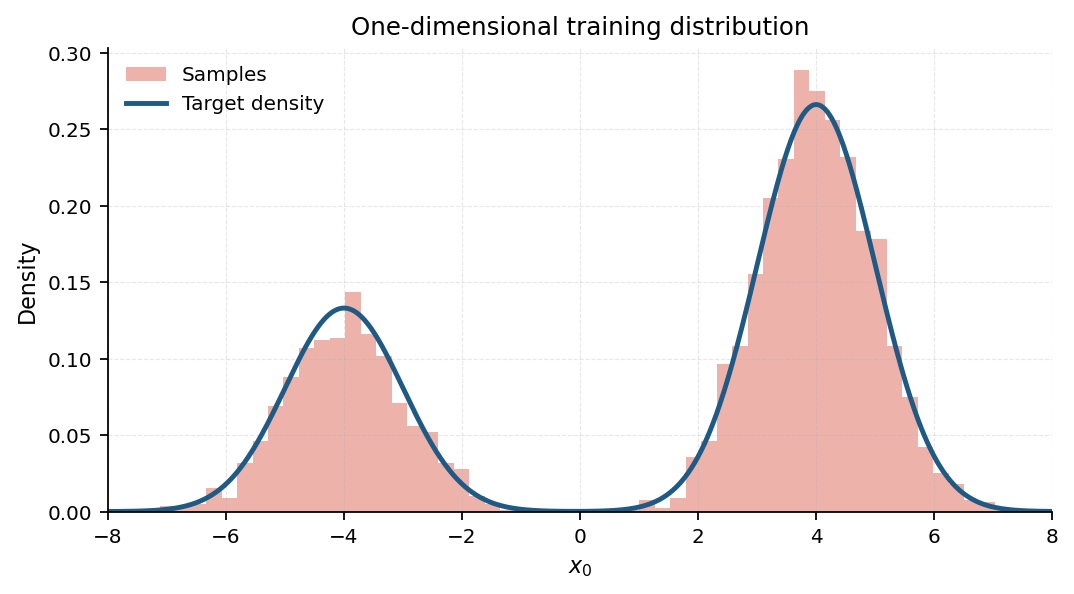
\includegraphics[width=0.70\textwidth]{figures/ch3/diffusion_1d_dataset.png}
    \caption{One-dimensional toy distribution used to illustrate diffusion.
    The histogram represents samples drawn from a bimodal Gaussian mixture,
    while the curve shows the corresponding probability density.}
    \label{fig:diffusion_1d_dataset}
\end{figure}

%%%%%%%%%%%%%%%%%%%%%%%%%%%%%%%%%%%%%%%%%%%%%%%%%%%%%%%%%%%%%%

\subsection{Forward diffusion process}

Following the unified framework introduced by \citep{Song2021SDE}, diffusion models can be interpreted as stochastic processes that progressively transform the data distribution into a simple tractable distribution. Let

\begin{equation}
\mathbf{x}_0 \sim p_{\mathrm{data}}(\mathbf{x}_0)
\end{equation}


denote a sample drawn from the unknown distribution of RTI density fields. The forward diffusion process is defined as a continuous-time stochastic differential equation (SDE)

\begin{equation}
d\mathbf{x}
=
\mathbf{f}(\mathbf{x},t)dt
+
g_{\mathrm{diff}}(t)d\mathbf{w}
\end{equation}
where $t\in[0,\mathds{1}]$, $\mathbf{w}$ denotes a standard Wiener process, and
\[
\mathbf{f}:\mathbb{R}^{d}\times[0,\mathds{1}]\to\mathbb{R}^{d}
\quad\text{and}\quad
g_{\mathrm{diff}}:[0,\mathds{1}]\to\mathbb{R}_{+}
\]
are respectively the drift coefficient and the diffusion coefficient,
which controls the intensity of the injected noise \citep{Song2021SDE}.

The objective of this process is to progressively destroy the structure present in the data. As time increases, the probability distribution $(p_t(\mathbf{x}))$ evolves from the complex data distribution $(p_{\mathrm{data}})$ toward a simple prior distribution that is chosen as a standard Gaussian,

\begin{equation}
p_{\mathds{1}}(\mathbf{x})
\approx
\mathcal{N}(\mathbf{0},\mathbf{I})
\end{equation}

Several choices of forward SDEs are possible. In this work, the implementation is based on the continuous variance-preserving (VP) SDE used in score-based generative modeling \citep{Song2021SDE}. In this case, the forward process can be written as

\begin{equation}
d\mathbf{x}
=
-\frac{1}{2}\beta(t)\mathbf{x}\,dt
+
\sqrt{\beta(t)}\,d\mathbf{w}
\end{equation}

where $(\beta(t))$ controls the noise schedule. In the implemented SGM,
\[
\beta(t)=\beta_{\min}+(\beta_{\max}-\beta_{\min})t,
\qquad t\in[0,\mathds{1}],
\]
with positive bounds satisfying $0<\beta_{\min}\leq\beta_{\max}$.

The implementation used during training does not simulate the forward SDE by Euler--Maruyama. It samples the exact marginal distribution at a continuous time $t\in[0,\mathds{1}]$. Defining
\begin{equation}
\bar{\alpha}(t)
=
\exp\left(-\int_0^t \beta(s)\,ds\right),
\end{equation}
the noisy sample at any diffusion time can be obtained directly through

\begin{equation}
\mathbf{x}_t
=
\sqrt{\bar{\alpha}(t)}\,\mathbf{x}_0
+
\sqrt{1-\bar{\alpha}(t)}\,
\boldsymbol{\epsilon}
\qquad
\boldsymbol{\epsilon}
\sim
\mathcal{N}(\mathbf{0},\mathbf{I})
\label{eq:x_t}
\end{equation}

\begin{compactproof}[title={Proof}]
\proofstep{Idea} Integrate $d\mathbf{x}$ without the diffusion term to get the
deterministic part, then add the stochastic contribution.

\proofstep{Linear ODE} With $d\mathbf{w}=0$, the deterministic dynamics is
\[
    \frac{d\mathbf{x}}{dt}
    =
    -\frac{1}{2}\beta(t)\mathbf{x}.
\]
Its solution is
\[
    \mathbf{x}(t)
    =
    \mathbf{x}_0
    \, e^{
        -\frac{1}{2}\int_0^t \beta(s)\,ds}.
\]
Thus one may define
\[
    \alpha(t)
    = e^{
        -\frac{1}{2}\int_0^t \beta(s)\,ds},
    \qquad
    \mathbf{x}(t)=\alpha(t)\mathbf{x}_0.
\]

\proofstep{Stochastic term} For the stochastic part, set
$\mathbf{y}(t)=\alpha(t)^{-1}\mathbf{x}(t)$. Since $\alpha(t)$ is deterministic,
Ito's product rule gives
\[
    d\mathbf{y}
    =
    \alpha(t)^{-1}d\mathbf{x}
    +
    \mathbf{x}\,d(\alpha(t)^{-1}).
\]
Substituting the SDE and the derivative of $\alpha(t)^{-1}$ cancels the drift,
which yields
\[
    d\mathbf{y}
    =
    \alpha(t)^{-1}\sqrt{\beta(t)}\,d\mathbf{w}.
\]

Thus, to recover $\mathbf{x}(t)$, one can integrate the stochastic term and multiply by $\alpha(t)$:
\begin{align*}
    \int_{0}^{t} dy &= \int_{0}^{t} \alpha(s)^{-1}\sqrt{\beta(s)}\,d\mathbf{w} \\
    \Rightarrow x(t) &= \alpha(t) \, x_0 + \alpha(t) \int_{0}^{t} \alpha(s)^{-1}\sqrt{\beta(s)}\,d\mathbf{w}
\end{align*}

\proofstep{Distribution} The integral of the stochastic term is a Gaussian random variable with mean zero and variance
\begin{align*}
    \text{Var}\left(\alpha(t) \int_{0}^{t} \alpha(s)^{-1}\sqrt{\beta(s)}\,d\mathbf{w}\right)
    &= \alpha(t)^2 \int_{0}^{t} (\alpha(s)^{-1}\sqrt{\beta(s)})^2 ds \\
    &= \alpha(t)^2 \int_{0}^{t} \alpha(s)^{-2} \beta(s) ds \\
    &= \alpha(t)^2 \left( \frac{1}{\alpha(t)^2} -1 \right) \\
    &= 1 - \alpha(t)^2
\end{align*}


\proofstep{Conclusion} By combining the deterministic and stochastic parts, we obtain the final expression for $\mathbf{x}_t$ setting $\bar{\alpha}(t) = \alpha(t)^2$:
\begin{equation*}
\boxed{
    \mathbf{x}_t
    =
    \sqrt{\bar{\alpha}(t)}\,\mathbf{x}_0
    +
    \sqrt{1-\bar{\alpha}(t)}\,\boldsymbol{\epsilon},
    \qquad
    \boldsymbol{\epsilon}\sim\mathcal{N}(\mathbf{0},\mathbf{I}).
}
\end{equation*}
\qedcompact
\end{compactproof}

By showing that the forward process can be solved analytically, the proof above also provides a practical way to generate noisy samples at any diffusion time. The same result can be obtained by iteratively applying the discrete transition kernel, but the closed-form expression is more efficient and avoids the accumulation of numerical errors.

This mechanism is illustrated Figure~\ref{fig:diff1d} in
one dimension by a bimodal distribution: its two modes progressively
merge until the samples become approximately Gaussian. The same principle
applies to RTI fields, although their probability distribution lies in a much
higher-dimensional space and cannot be represented by a simple histogram.

\begin{figure}[H]
    \centering
    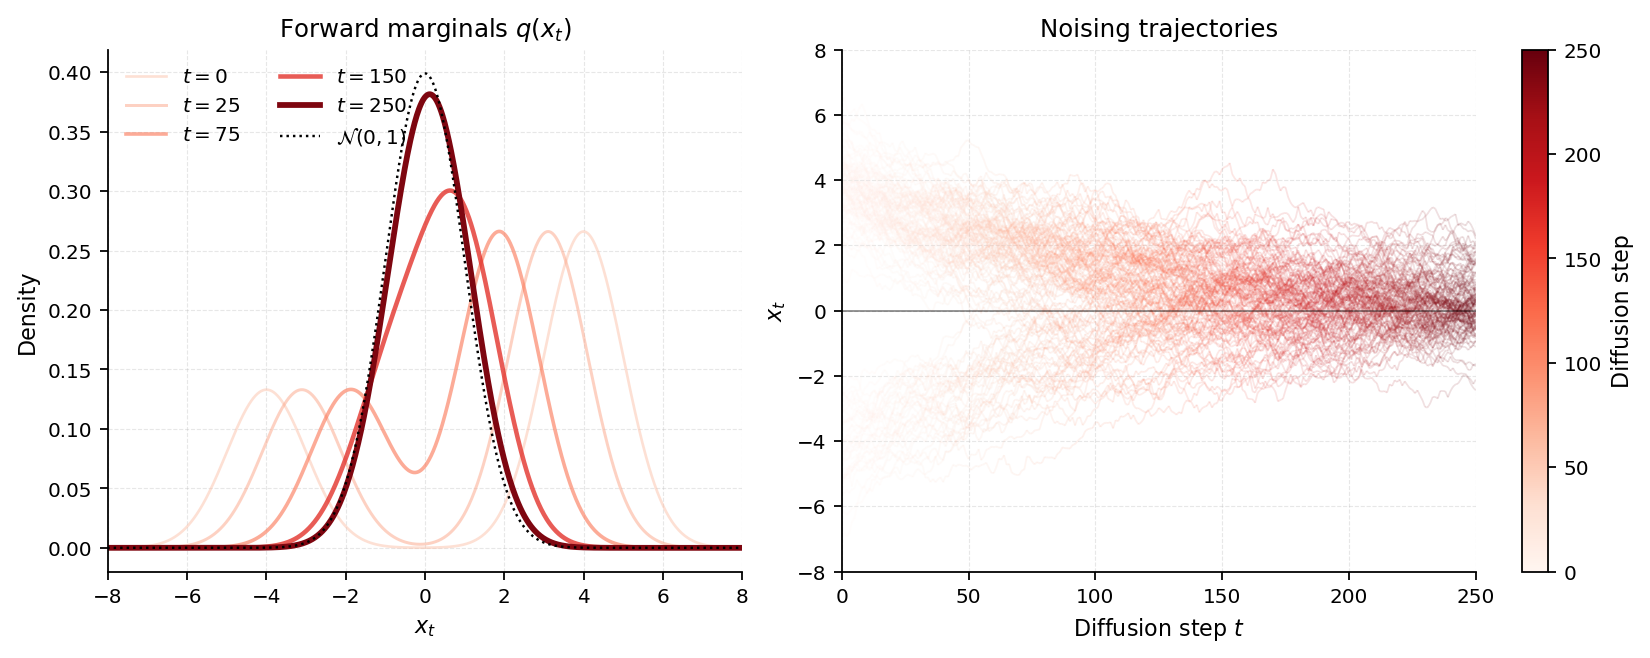
\includegraphics[width=0.95\textwidth]{figures/ch3/diffusion_1d_forward.png}
    \caption{Forward diffusion in one dimension. Left: evolution of the noisy
    marginal density $p_t(\mathbf{x})$ for several diffusion times. Right: trajectories
    of individual samples during the Markov noising process.}
    \label{fig:diff1d}
\end{figure}

%%%%%%%%%%%%%%%%%%%%%%%%%%%%%%%%%%%%%%%%%%%%%%%%%%%%%%%%%%%%%%

\subsection{Learning the Reverse Process Through the Score}

While the forward process is known analytically, the reverse evolution that transforms Gaussian noise back into realistic samples is generally intractable. A central result established by \citep{ANDERSON1982313} and exploited by \citep{Song2021SDE} is that the reverse-time dynamics of the diffusion process is itself governed by a stochastic differential equation,

\begin{equation}
d\mathbf{x}
=
\left[
\mathbf{f}(\mathbf{x},t)
-
g_{\mathrm{diff}}(t)^2
\nabla_{\mathbf{x}}
\log p_t(\mathbf{x})
\right]dt
+
g_{\mathrm{diff}}(t)d\bar{\mathbf{w}}, \quad {\scriptstyle \text{where $\bar{\mathbf{w}}$ is a reverse-time Wiener process.}}
\end{equation}

\begin{compactproof}[title={Proof}]
\proofstep{Idea} Associate the forward process with a Fokker-Planck equation and then derive the reverse-time SDE from it.
\proofstep{Step 1} Consider the forward SDE
\begin{equation*}
d\mathbf{x}
=
\mathbf{f}(\mathbf{x},t)dt
+
g_{\mathrm{diff}}(t)d\mathbf{w},
\end{equation*}
where $\mathbf{w}$ is a Wiener process. The corresponding Fokker-Planck equation describes the evolution of the probability density $p_t(\mathbf{x})$ of $\mathbf{x}$ at time $t$:
\begin{equation*}
\frac{\partial p_t(\mathbf{x})}{\partial t}
=
-\nabla_{\mathbf{x}}\cdot\left[\mathbf{f}(\mathbf{x},t)p_t(\mathbf{x})\right]
+
\frac{1}{2}g_{\mathrm{diff}}(t)^2\nabla_{\mathbf{x}}^2p_t(\mathbf{x}).
\end{equation*}
Let thus derive the  Fokker-Planck equation for $\tau = \mathds{1}-t$ and $q_t(\mathbf{x})=p_{\tau}(\mathbf{x})$ the probability density of $\mathbf{y}(t)=\mathbf{x}(\tau)$:
\begin{align*}
    \partial q_t(\mathbf{x})
    &=
    -\partial p_{\tau}(\mathbf{x})\\
    &=
    \nabla_{\mathbf{x}}\cdot\left[\mathbf{f}(\mathbf{x},\tau)p_{\tau}(\mathbf{x})\right]
    -
    \frac{1}{2}g_{\mathrm{diff}}(\tau)^2\nabla_{\mathbf{x}}^2p_{\tau}(\mathbf{x})\\
    &=
    \nabla_{\mathbf{x}}\cdot\left[\mathbf{f}(\mathbf{x},\tau)q_t(\mathbf{x})\right]
    +
    \left(-1+\frac{1}{2}\right)g_{\mathrm{diff}}(\tau)^2\nabla_{\mathbf{x}}^2q_t(\mathbf{x})\\
    &=
    \nabla_{\mathbf{x}}\cdot\left[\left(\mathbf{f}(\mathbf{x},\tau)-g_{\mathrm{diff}}(\tau)^2\frac{\nabla_{\mathbf{x}}q_t(\mathbf{x})}{q_t(\mathbf{x})}\right)q_t(\mathbf{x})\right]
    +
    \frac{1}{2}g_{\mathrm{diff}}(\tau)^2\nabla_{\mathbf{x}}^2q_t(\mathbf{x}).  \\
    &=
    \nabla_{\mathbf{x}}\cdot\left[\left(\mathbf{f}(\mathbf{x},\tau)-g_{\mathrm{diff}}(\tau)^2\nabla_{\mathbf{x}}\log q_t(\mathbf{x})\right)q_t(\mathbf{x})\right]
    +
    \frac{1}{2}g_{\mathrm{diff}}(\tau)^2\nabla_{\mathbf{x}}^2q_t(\mathbf{x}) \quad 
    {\scriptstyle \text{with:} \frac{\nabla_{\mathbf{x}}q_t(\mathbf{x})}{q_t(\mathbf{x})} = \nabla_{\mathbf{x}}\log q_t(\mathbf{x}) } \\
    &= 
    - \nabla_{\mathbf{x}}\cdot\left[\left(-\mathbf{f}(\mathbf{x},\tau)+g_{\mathrm{diff}}(\tau)^2\nabla_{\mathbf{x}}\log q_t(\mathbf{x})\right)q_t(\mathbf{x})\right]
    +
    \frac{1}{2}g_{\mathrm{diff}}(\tau)^2\nabla_{\mathbf{x}}^2q_t(\mathbf{x}).
\end{align*}

The last line is the Fokker-Planck equation corresponding to the reverse-time SDE

\begin{equation*}
\boxed{
d\mathbf{y}
=
\left[
\mathbf{f}(\mathbf{y},\tau)
-
g_{\mathrm{diff}}(\tau)^2
\nabla_{\mathbf{y}}
\log q_t(\mathbf{y})
\right]dt
+
g_{\mathrm{diff}}(\tau)d\bar{\mathbf{w}}
}
\end{equation*}

where $\bar{\mathbf{w}}$ is a reverse-time Wiener process. Finally, we can replace $\tau$ with $\mathds{1}-t$ and $q_t(\mathbf{x})$ with $p_{\mathds{1}-t}(\mathbf{x})$ to obtain the reverse-time SDE in terms of the original time variable $t$ and the original probability density $p_t(\mathbf{x})$.     

\end{compactproof}

The score $\mathbf{s}(\mathbf{x},t) \approx \nabla_{\mathbf{x}}\log p_t(\mathbf{x})$ corresponds to the gradient of the logarithmic probability density. Geometrically, it points toward regions of higher probability and therefore indicates how a noisy sample should be displaced in order to become more representative of the underlying data distribution. It is now required to estimate the score with only a finite number of samples $(\mathbf{x}_{0},\mathbf{x}_{t})$ drawn from the forward diffusion process. Considering $\mathbf{x}_{t} = \alpha(t)\mathbf{x}_{0} + \sigma(t)\boldsymbol{\epsilon}$, with $\alpha(t)=\sqrt{\bar{\alpha}(t)}$, $\sigma(t)=\sqrt{1-\bar{\alpha}(t)}$, and $\boldsymbol{\epsilon} \sim \mathcal{N}(0, I)$ as shown in Equation~\ref{eq:x_t}, it is possible to rewrite the score as

\begin{equation}
    \mathbf{s}_{\theta}(\mathbf{x}_t,t)
    \approx
    \nabla_{\mathbf{x}_t}\log p_t(\mathbf{x}_t)
    =
    \mathbb{E}[
        \nabla_{\mathbf{x}_t}\log p(\mathbf{x}_t|\mathbf{x}_0)
        \mid
        \mathbf{x}_t
    ]
\end{equation}

\begin{compactproof}[title={Proof}]
\proofstep{Idea}
Show that the marginal score $\nabla_{\mathbf{x}_t}\log p_t(\mathbf{x}_t)$, which is required to define the reverse-time diffusion process, can be written as the conditional expectation of the transition score
$\nabla_{\mathbf{x}_t}\log p_{t\mid 0}(\mathbf{x}_t\mid \mathbf{x}_0)$.
Since the transition distribution is chosen explicitly, its score can be computed and used as a training target.

\proofstep{Step 1}
Let $p_0(\mathbf{x}_0)$ denote the data distribution and let
$p_{t\mid 0}(\mathbf{x}_t\mid \mathbf{x}_0)$ denote the transition density of the forward diffusion process. The marginal density at time $t$ is
\begin{equation*}
p_t(\mathbf{x}_t)
=
\int
p_{t\mid 0}(\mathbf{x}_t\mid \mathbf{x}_0)
p_0(\mathbf{x}_0)
\,d\mathbf{x}_0.
\end{equation*}

Taking the gradient with respect to $\mathbf{x}_t$ gives
\begin{align*}
\nabla_{\mathbf{x}_t}p_t(\mathbf{x}_t)
&=
\nabla_{\mathbf{x}_t}
\int
p_{t\mid 0}(\mathbf{x}_t\mid \mathbf{x}_0)
p_0(\mathbf{x}_0)
\,d\mathbf{x}_0
\\
&=
\int
\nabla_{\mathbf{x}_t}
p_{t\mid 0}(\mathbf{x}_t\mid \mathbf{x}_0)
p_0(\mathbf{x}_0)
\,d\mathbf{x}_0.
\end{align*}

Dividing by $p_t(\mathbf{x}_t)$ yields
\begin{align*}
\nabla_{\mathbf{x}_t}\log p_t(\mathbf{x}_t)
&=
\frac{
\nabla_{\mathbf{x}_t}p_t(\mathbf{x}_t)
}{
p_t(\mathbf{x}_t)
}
\\
&=
\int
\frac{
\nabla_{\mathbf{x}_t}
p_{t\mid 0}(\mathbf{x}_t\mid \mathbf{x}_0)
}{
p_t(\mathbf{x}_t)
}
p_0(\mathbf{x}_0)
\,d\mathbf{x}_0.
\end{align*}

Using
\begin{equation*}
\nabla_{\mathbf{x}_t}
p_{t\mid 0}(\mathbf{x}_t\mid \mathbf{x}_0)
=
p_{t\mid 0}(\mathbf{x}_t\mid \mathbf{x}_0)
\nabla_{\mathbf{x}_t}
\log p_{t\mid 0}(\mathbf{x}_t\mid \mathbf{x}_0),
\end{equation*}
we obtain
\begin{align*}
\nabla_{\mathbf{x}_t}\log p_t(\mathbf{x}_t)
&=
\int
\nabla_{\mathbf{x}_t}
\log p_{t\mid 0}(\mathbf{x}_t\mid \mathbf{x}_0)
\frac{
p_{t\mid 0}(\mathbf{x}_t\mid \mathbf{x}_0)
p_0(\mathbf{x}_0)
}{
p_t(\mathbf{x}_t)
}
\,d\mathbf{x}_0.
\end{align*}

By Bayes' rule,
\begin{equation*}
p_{0\mid t}(\mathbf{x}_0\mid \mathbf{x}_t)
=
\frac{
p_{t\mid 0}(\mathbf{x}_t\mid \mathbf{x}_0)
p_0(\mathbf{x}_0)
}{
p_t(\mathbf{x}_t)
}.
\end{equation*}

Therefore,
\begin{align*}
\nabla_{\mathbf{x}_t}\log p_t(\mathbf{x}_t)
&=
\int
\nabla_{\mathbf{x}_t}
\log p_{t\mid 0}(\mathbf{x}_t\mid \mathbf{x}_0)
p_{0\mid t}(\mathbf{x}_0\mid \mathbf{x}_t)
\,d\mathbf{x}_0
\\
&=
\mathbb{E}_{\mathbf{x}_0\sim
p_{0\mid t}(\cdot\mid\mathbf{x}_t)}
\left[
\nabla_{\mathbf{x}_t}
\log p_{t\mid 0}(\mathbf{x}_t\mid \mathbf{x}_0)
\right]
\\
&=
\mathbb{E}
\left[
\nabla_{\mathbf{x}_t}
\log p_{t\mid 0}(\mathbf{x}_t\mid \mathbf{x}_0)
\,\middle|\,
\mathbf{x}_t
\right].
\end{align*}

Hence,
\begin{equation*}
\boxed{
\nabla_{\mathbf{x}_t}\log p_t(\mathbf{x}_t)
=
\mathbb{E}
\left[
\nabla_{\mathbf{x}_t}
\log p_{t\mid 0}(\mathbf{x}_t\mid \mathbf{x}_0)
\,\middle|\,
\mathbf{x}_t
\right].
}
\end{equation*}
\end{compactproof}




Consider now a Gaussian forward perturbation kernel with mean $\alpha(t)\mathbf{x}_0$ and variance $\sigma(t)^2\mathbf{I}$, where $\alpha(t)=\sqrt{\bar{\alpha}(t)}$ and $\sigma(t)=\sqrt{1-\bar{\alpha}(t)}$ are known functions of time from Equation~\eqref{eq:x_t}. The forward process can be written as
\begin{equation*}
\mathbf{x}_t
=
\alpha(t)\mathbf{x}_0
+
\sigma(t)\boldsymbol{\epsilon},
\qquad
\boldsymbol{\epsilon}\sim\mathcal{N}(\mathbf{0},\mathbf{I}).
\end{equation*}
Leading to the transition density
\begin{equation}
    \nabla_{\mathbf{x}_t}
    \log p_{t\mid 0}(\mathbf{x}_t\mid\mathbf{x}_0)
    =
    -\frac{\boldsymbol{\epsilon}}{\sigma(t)},
\end{equation}


\begin{compactproof}[title={Proof}]
\proofstep{Idea}
Compute the logarithm of the Gaussian transition density and take its gradient with respect to $\mathbf{x}_t$.
Conditionally on $\mathbf{x}_0=\mathbf{x}_0$, one has
\begin{equation*}
p_{t\mid 0}(\mathbf{x}_t\mid\mathbf{x}_0)
=
\mathcal{N}
\left(
\mathbf{x}_t;
\alpha(t)\mathbf{x}_0,
\sigma(t)^2\mathbf{I}
\right).
\end{equation*}

Its logarithm is, up to a term independent of $\mathbf{x}_t$,
\begin{equation*}
\log p_{t\mid 0}(\mathbf{x}_t\mid\mathbf{x}_0)
=
-\frac{1}{2\sigma(t)^2}
\left\|
\mathbf{x}_t-\alpha(t)\mathbf{x}_0
\right\|^2
+
C(t,\mathbf{x}_0).
\end{equation*}

Consequently,
\begin{align*}
&\nabla_{\mathbf{x}_t}
\log p_{t\mid 0}(\mathbf{x}_t\mid\mathbf{x}_0)
=
-\frac{
\mathbf{x}_t-\alpha(t)\mathbf{x}_0
}{
\sigma(t)^2
}
\\
\Rightarrow\qquad
&
\boxed{
\nabla_{\mathbf{x}_t}
\log p_{t\mid 0}(\mathbf{x}_t\mid\mathbf{x}_0)
=
-\frac{\boldsymbol{\epsilon}}{\sigma(t)}
}
\qquad
{\scriptstyle
\text{since }
\mathbf{x}_t-\alpha(t)\mathbf{x}_0
=
\sigma(t)\boldsymbol{\epsilon}.
}
\end{align*}

\end{compactproof}

Or $\sigma(t)$ is known and $\boldsymbol{\epsilon}$ can be estimated by a neural network $\boldsymbol{\epsilon}_{\theta}(\mathbf{x}_t,t)$, which leads to the following training objective:

\begin{equation}
    \boxed{
    \mathcal{L}_{\mathrm{simple}}(\theta)
    =
    \mathbb{E}_{t,\mathbf{x}_0,\boldsymbol{\epsilon}}
    \left[
        \left\|
            \boldsymbol{\epsilon}
            -
            \boldsymbol{\epsilon}_{\theta}(\mathbf{x}_t,t)
        \right\|_2^2
    \right].
    }
    \label{eq:simple_noise_loss}
\end{equation}

%%%%%%%%%%%%%%%%%%%%%%%%%%%%%%%%%%%%%%%%%%%%%%%%%%%%%%%%%%%%%%

\subsection{Sampling from the learned reverse process}
\label{subsec:sampling_reverse_process}

The training objective above provides an approximation of the score
$\nabla_{\mathbf{x}}\log p_t(\mathbf{x})$ for every diffusion time. It does
not, however, directly generate a new density field. Once the network has been
trained, sampling consists in replacing the unknown score in the reverse
process by its neural approximation and solving the resulting stochastic
differential equation numerically.

To remain consistent with the time reversal introduced in the previous proof,
let $ \tau = \mathds{1} - t$ and so $ \mathbf{y}_t = \mathbf{x}_{\tau} $ and $ q_t(\mathbf{y}) = p_{\tau}(\mathbf{y}) $. The reverse process is then written with a time variable increasing from $ \tau = 0 $ to $ \tau = \mathds{1} $ as
\begin{equation}
    d\mathbf{y}
    =
    \left[
        -\mathbf{f}(\mathbf{y},\tau)
        +g_{\mathrm{diff}}(\tau)^2
        \nabla_{\mathbf{y}}\log p_{\tau}(\mathbf{y})
    \right]dt
    +
    g_{\mathrm{diff}}(\tau)d\overline{\mathbf{w}}.
    \label{eq:reverse_sde_increasing_time}
\end{equation}
At the beginning of the reverse process, we have $ \mathbf{y}_0=\mathbf{x}_{\mathds{1}} \sim p_{\mathds{1}} \approx \mathcal{N}(\mathbf{0},\mathbf{I}) $ and if Equation~\eqref{eq:reverse_sde_increasing_time} were solved using the exact
score, its terminal random variable would satisfy $ \mathbf{y}_{\mathds{1}}\sim p_0=p_{\mathrm{data}} $.
In practice, the exact score is replaced by the learned approximation
$\mathbf{s}_{\theta}$, which gives
\begin{equation}
    d\mathbf{y}
    =
    \mathbf{b}_{\theta}(\mathbf{y},t)dt
    +g_{\mathrm{diff}}(\tau)d\overline{\mathbf{w}},
    \label{eq:learned_reverse_sde_sampling}
\end{equation}
\vspace{-5pt}
\begin{equation*}
    \text{with,} \quad
    \mathbf{b}_{\theta}(\mathbf{y},t)
    =
    -\mathbf{f}(\mathbf{y},\tau)
    +g_{\mathrm{diff}}(\tau)^2
    \mathbf{s}_{\theta}(\mathbf{y},\tau).
    \label{eq:learned_reverse_drift_sampling}
\end{equation*}
Using the noise-prediction parameterization
$\mathbf{s}_{\theta}(\mathbf{x}_t,t)
=-\boldsymbol{\epsilon}_{\theta}(\mathbf{x}_t,t)/\sigma(t)$, the drift can
also be evaluated directly from the output of the trained network.

Equation~\eqref{eq:learned_reverse_sde_sampling} generally has no closed-form
solution because its drift depends on the nonlinear neural network. A temporal
grid
\begin{equation}
    0=t_0<t_1<\cdots<t_{N_{\mathrm{step}}}=\mathds{1},
    \qquad
    \Delta t_n=t_{n+1}-t_n,
\end{equation}
is therefore introduced. The Wiener increment over one time step is sampled as
\begin{equation}
    \Delta\overline{\mathbf{w}}_n
    =
    \sqrt{\Delta t_n}\,\mathbf{z}_n,
    \qquad
    \mathbf{z}_n\sim\mathcal{N}(\mathbf{0},\mathbf{I}).
\end{equation}
A direct Euler--Maruyama discretization would give
\begin{equation}
    \mathbf{y}_{n+1}
    =
    \mathbf{y}_n
    +\Delta t_n\mathbf{b}_{\theta}(\mathbf{y}_n,t_n)
    +g_{\mathrm{diff}}(\mathds{1}-t_n)\sqrt{\Delta t_n}\,\mathbf{z}_n.
    \label{eq:euler_maruyama_sampling}
\end{equation}
This expression makes the role of the trained network explicit: at each noise
level, the score estimate modifies the drift of the reverse diffusion and
therefore determines the direction in which the current noisy sample evolves.
The Gaussian term preserves the stochastic nature of the reverse process.

In this work, the integration is performed using a predictor--corrector scheme
of Heun type. First, an Euler prediction is computed,
\begin{equation}
    \widetilde{\mathbf{y}}_{n+1}
    =
    \mathbf{y}_n
    +\Delta t_n\mathbf{b}_{\theta}(\mathbf{y}_n,t_n)
    +g_{\mathrm{diff}}(\mathds{1}-t_n)\sqrt{\Delta t_n}\,\mathbf{z}_n.
    \label{eq:heun_sampling_predictor}
\end{equation}
The drift is then evaluated again at the predicted state, and the two drift
estimates are averaged,
\begin{equation}
\begin{aligned}
    \mathbf{y}_{n+1}
    ={}&
    \mathbf{y}_n
    +\frac{\Delta t_n}{2}
    \left[
        \mathbf{b}_{\theta}(\mathbf{y}_n,t_n)
        +
        \mathbf{b}_{\theta}
        (\widetilde{\mathbf{y}}_{n+1},t_{n+1})
    \right]
    \\
    &+
    g_{\mathrm{diff}}(\mathds{1}-t_n)\sqrt{\Delta t_n}\,\mathbf{z}_n.
    \label{eq:heun_sampling_corrector}
\end{aligned}
\end{equation}
The same Gaussian realization $\mathbf{z}_n$ is used in the prediction and
correction. Compared with Euler--Maruyama, the Heun correction accounts for the
variation of the learned drift over the time step, at the cost of a second
evaluation of the neural network.

Starting from $\mathbf{y}_0\sim\mathcal{N}(\mathbf{0},\mathbf{I})$ and
repeating these updates for $n=0,\ldots,N_{\mathrm{step}}-1$ produces the final state
$\mathbf{y}_{N_{\mathrm{step}}}$. Since $\mathbf{y}_{N_{\mathrm{step}}}$ approximates a sample from $p_0$, it is
interpreted as a newly generated RTI density field. Repeating the procedure
with independent initial Gaussian samples and independent Wiener increments
produces an ensemble whose distribution approximates
$p_{\mathrm{data}}$.

This behavior is illustrated in
Figure~\ref{fig:diffusion_1d_reverse_score}. In the one-dimensional example, the
score is represented by arrows along the $x$ axis. At each diffusion time, the
arrows point in the direction of increasing $p_t$. Near $t=\mathds{1}$, they mostly
point toward the origin because the distribution is nearly Gaussian. As the
reverse process approaches $t=0$, the central region becomes unstable and the
score directs samples toward one of the two modes of the original bimodal
distribution. The reverse process can therefore be interpreted as a gradual
transport of probability mass from a simple Gaussian prior toward the regions
occupied by the data.

\begin{figure}[H]
    \centering
    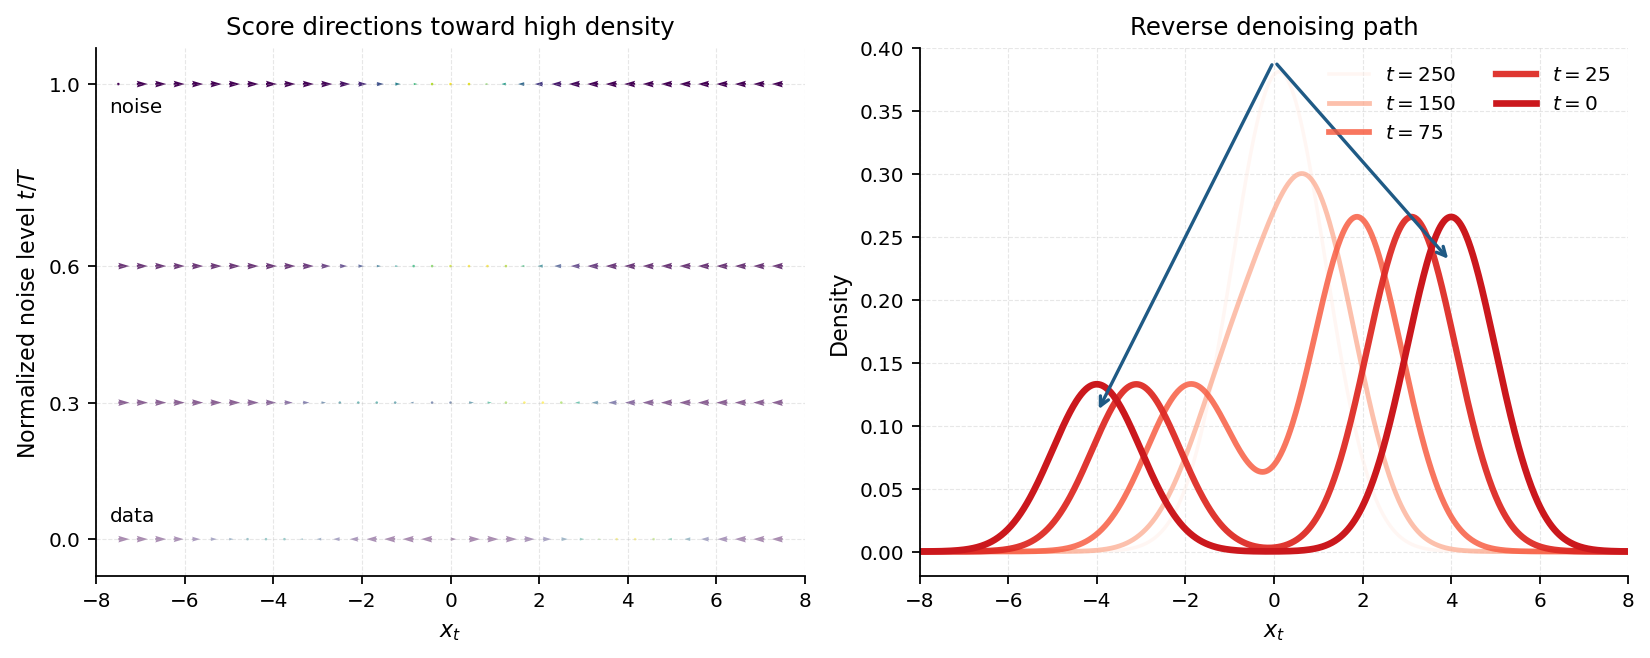
\includegraphics[width=0.95\textwidth]{figures/ch3/diffusion_1d_reverse_score.png}
    \caption{Score-based reverse process in the one-dimensional example. Left:
    score directions for several noise levels. Right: reverse denoising viewed
    as the transformation of the Gaussian prior back into the bimodal data
    distribution.}
    \label{fig:diffusion_1d_reverse_score}
\end{figure}

For RTI density fields, the same mechanism acts in a high-dimensional state
space. The network does not explicitly reconstruct an analytical expression
for $p_{\mathrm{data}}$. Instead, it learns the local vector field required to
transport noisy states toward regions of high probability at every noise level.
Repeated numerical integration of these learned directions produces an
ensemble of fields whose distribution approximates the distribution of the DNS
dataset.

%%%%%%%%%%%%%%%%%%%%%%%%%%%%%%%%%%%%%%%%%%%%%%%%%%%%%%%%%%%%%%
%%%%%%%%%%%%%%%%%%%%%%%%%%%%%%%%%%%%%%%%%%%%%%%%%%%%%%%%%%%%%%

\subsection{Conditional diffusion models}

The unconditional formulation above learns a marginal distribution
$p_{\theta}(\mathbf{x}_0)$ and generates samples from Gaussian noise alone.
Many practical settings instead require a \emph{conditional} model, where one
wants to sample from a distribution constrained by external information
$\mathbf{c}$. The objective then becomes

\begin{equation}
    p_{\theta}(\mathbf{x}_0 \mid \mathbf{c}).
\end{equation}

The conditioning variable may be a discrete label, a low-dimensional physical
parameter, or another structured signal. In the simple scalar example used in
the exploratory notebooks, $\mathbf{c}$ is a class label selecting one of two
signal families. In the wavelet setting that will be used in Chapter~4,
$\mathbf{c}$ is instead a coarse approximation coefficient field, while the
variable to be generated is the associated fine-scale detail field.

Figure~\ref{fig:conditional_diffusion_0d_forward} illustrates this idea on a
zero-dimensional toy problem. The marginal dataset is a mixture of several
Gaussian components, but each sample also carries a label $y\in\{0,1\}$. The
forward diffusion process still corrupts the scalar value $x_0$ with Gaussian
noise until the two conditional marginals become almost indistinguishable in
the noisy variable $x_t$. The crucial point is that the label is not diffused:
it remains available to the reverse model as side information.

\begin{figure}[H]
    \centering
    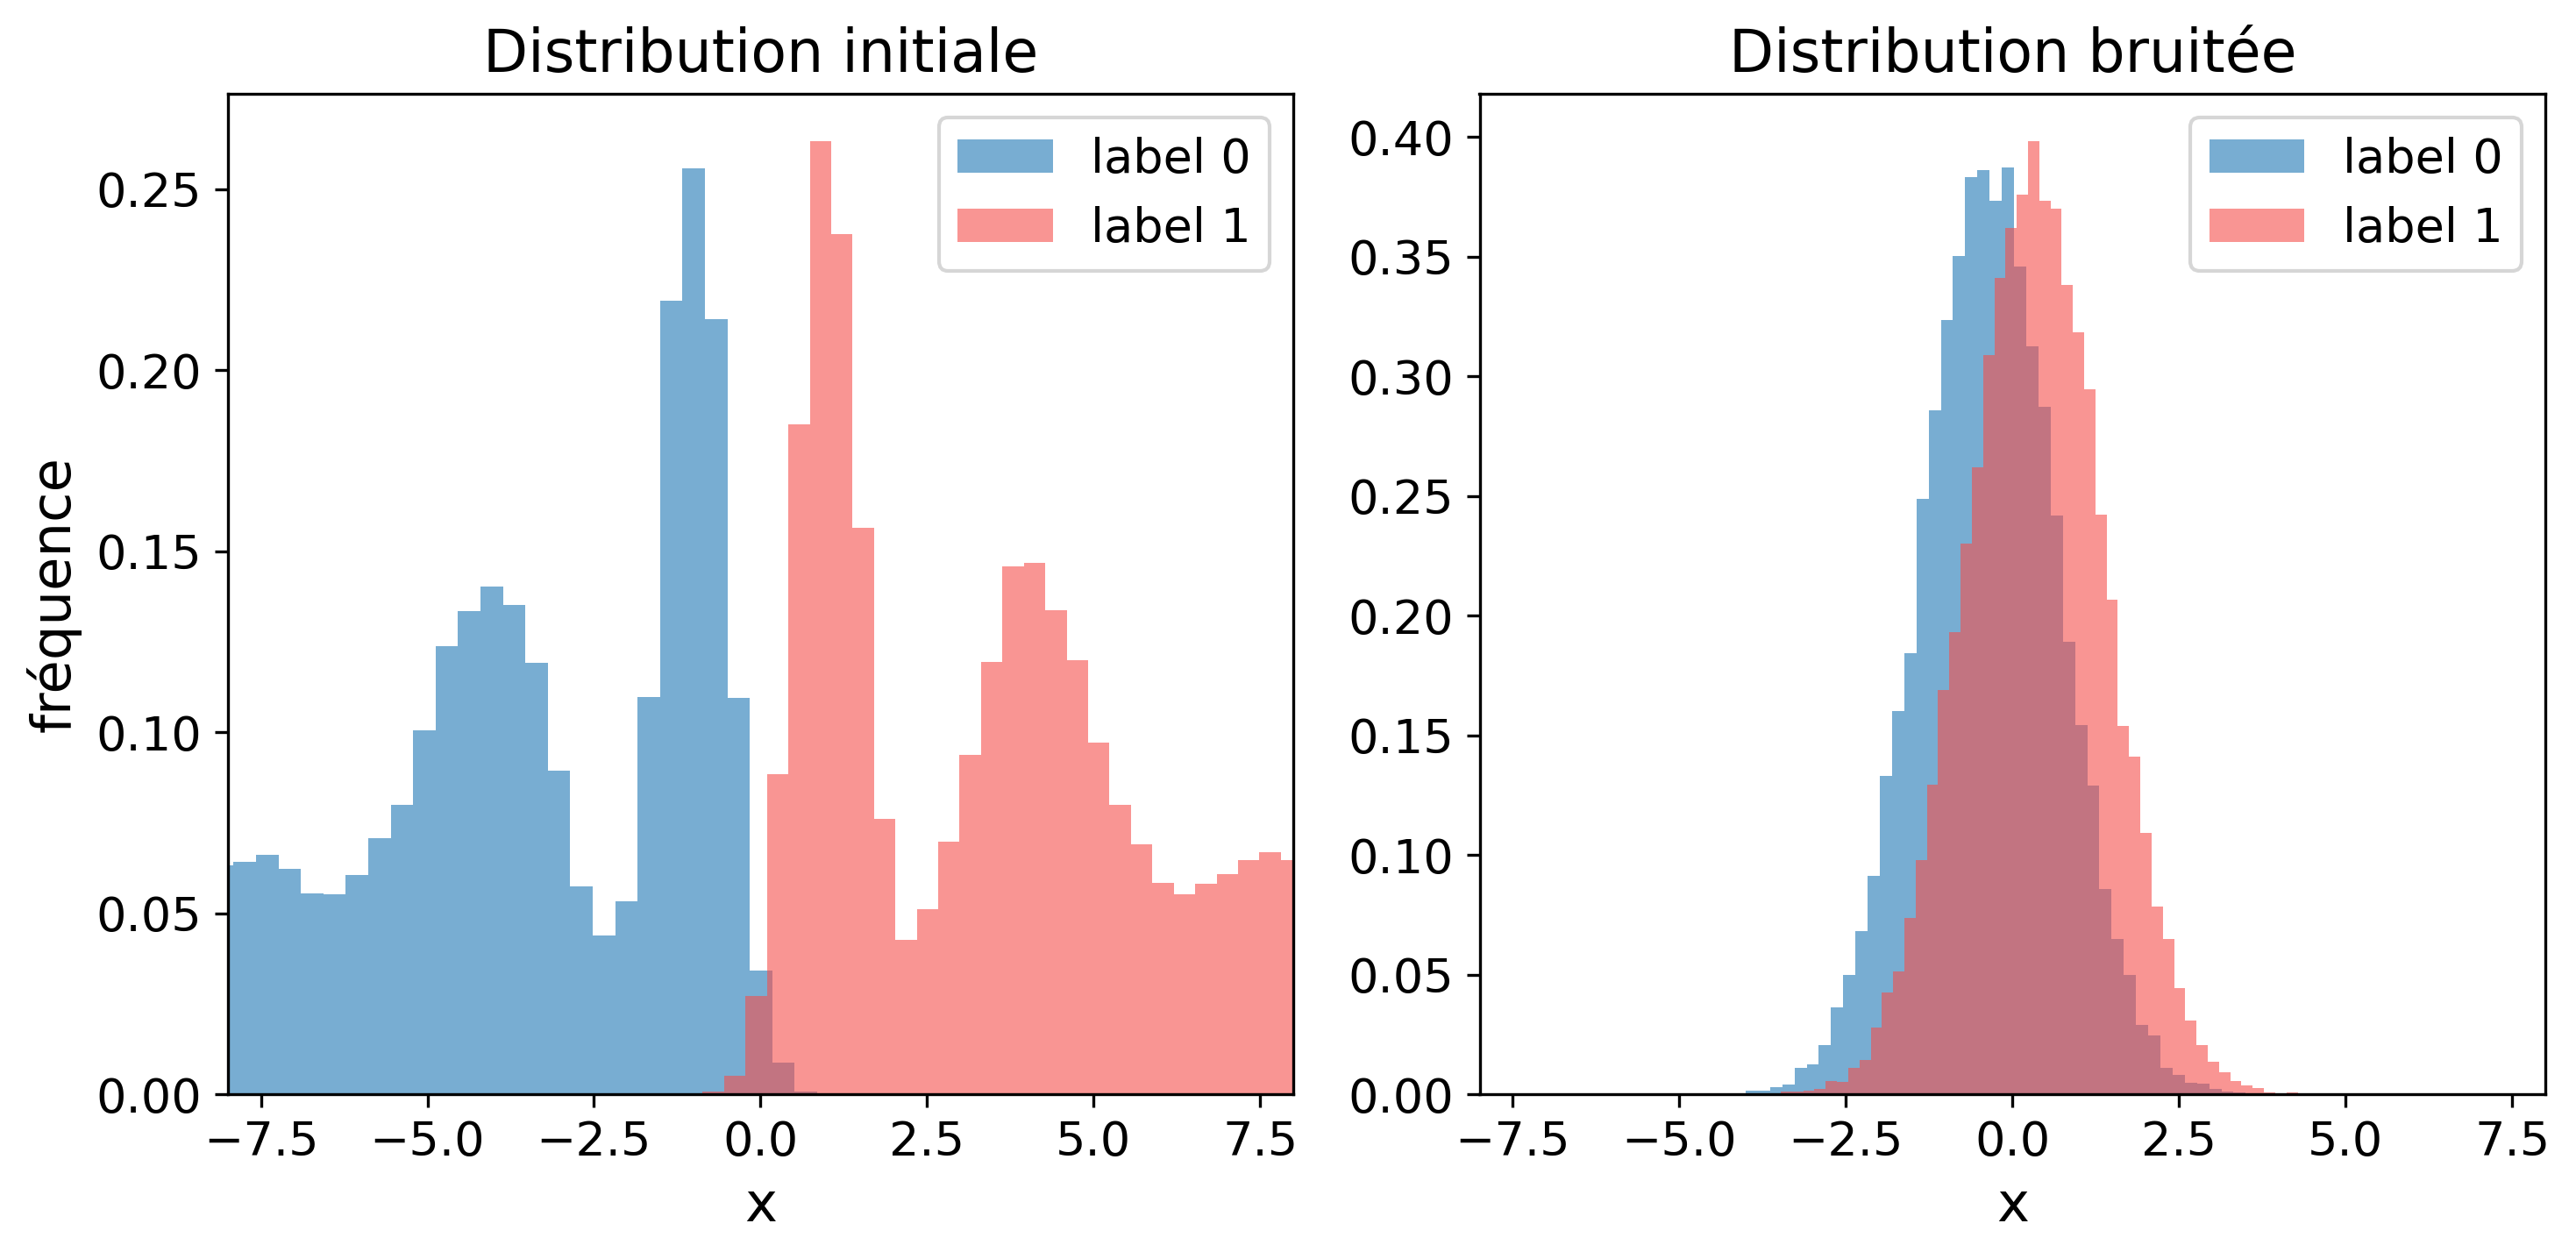
\includegraphics[width=0.85\textwidth]{figures/ch3/conditional_diffusion_0d_forward.png}
    \caption{Forward diffusion in a scalar conditional example. The initial distribution is split into two label-conditioned families. After sufficient noising, the two marginals collapse toward the same Gaussian-like distribution in $x_t$, while the label remains available as conditioning information.}
    \label{fig:conditional_diffusion_0d_forward}
\end{figure}

At the level of the forward process, nothing changes fundamentally: the target
variable is still progressively noised according to the same Markov chain. The
difference appears in the learned reverse model, which now predicts the noise
or the score using both the current noisy sample and the condition,

\begin{equation}
    \boldsymbol{\epsilon}_{\theta}(\mathbf{x}_t,t,\mathbf{c})
    \approx
    \boldsymbol{\epsilon}.
\end{equation}

The corresponding training objective becomes

\begin{equation}
    \mathcal{L}_{\mathrm{cond}}(\theta)
    =
    \mathbb{E}_{\mathbf{x}_0,\mathbf{c},t,\boldsymbol{\epsilon}}
    \left[
        \left\|
        \boldsymbol{\epsilon}
        -
        \boldsymbol{\epsilon}_{\theta}(\mathbf{x}_t,t,\mathbf{c})
        \right\|_2^2
    \right].
\end{equation}

This modification is conceptually simple but important. In an unconditional
model, the network must simultaneously infer the global organization and the
small-scale variability of the data. In a conditional model, part of this
uncertainty is removed by the condition. The model therefore learns a family of
conditional distributions rather than a single global distribution. When the
condition captures the low-frequency organization of the signal, the diffusion
model can focus its capacity on the residual variability compatible with that
coarse structure.

The practical effect is shown in
Figure~\ref{fig:conditional_diffusion_0d_generation}. A conditional network can
generate samples from the two label-conditioned distributions by changing only
the conditioning input. Without this information, an unconditional model would
only learn the marginal mixture and would not provide direct control over which
family is sampled. The conditioning therefore changes the learned reverse
transition from a single denoising field to a collection of denoising fields
indexed by $\mathbf{c}$.

\begin{figure}[H]
    \centering
    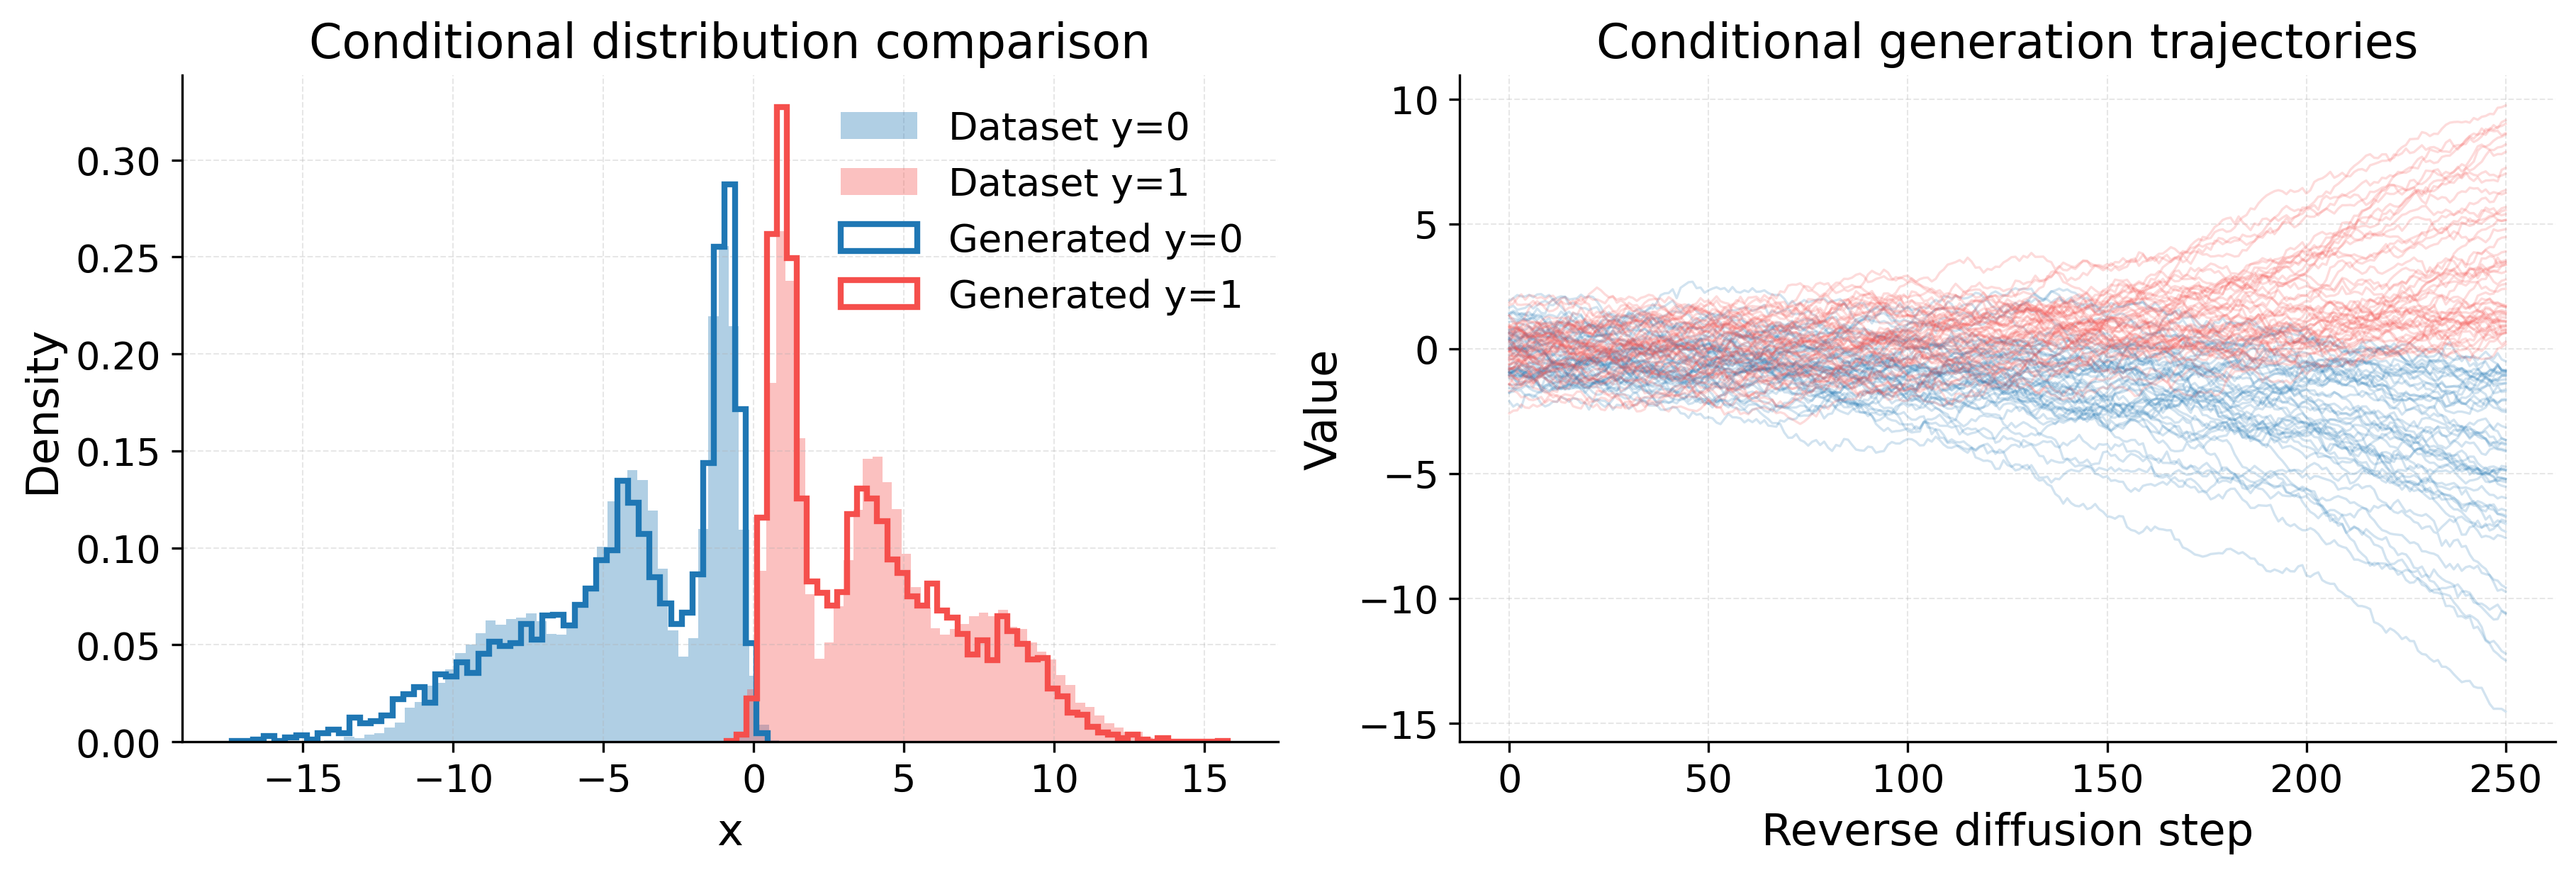
\includegraphics[width=0.95\textwidth]{figures/ch3/conditional_diffusion_0d_generation.png}
    \caption{Conditional generation in the scalar toy example. Left: generated samples reproduce the two target conditional distributions when the label is provided to the model. Right: reverse trajectories starting from Gaussian noise separate according to the prescribed condition.}
    \label{fig:conditional_diffusion_0d_generation}
\end{figure}

This coarse-to-fine factorization is especially relevant for multi-scale
physical fields. For a wavelet decomposition of a signal or image, one may
seek to model

\begin{equation}
    p(\mathbf{x})
    =
    p(LL,LH,HL,HH)
    =
    p(LL)\,p(LH,HL,HH\mid LL),
\end{equation}

where $LL$ denotes the approximation sub-band and $(LH,HL,HH)$ denote the
three directional detail sub-bands. In a deeper cascade, this factorization can be iterated
across scales, for example

\begin{equation}
    \begin{aligned}
    &p(LL^{(3)},LH^{(3)},HL^{(3)},HH^{(3)},LH^{(2)},HL^{(2)},HH^{(2)},LH^{(1)},HL^{(1)},HH^{(1)})\\
    &\qquad =
    p(LL^{(3)})
    \prod_{\ell=1}^{3}
    p(LH^{(\ell)},HL^{(\ell)},HH^{(\ell)}\mid LL^{(\ell)}),
    \end{aligned}
\end{equation}

which is precisely the logic explored in the multi-level wavelet notebooks.
The conceptual gain is that the model no longer needs to generate all scales at
once: coarse content is generated first, then progressively refined by
conditional detail models.

This decomposition does not make the problem trivial. Its usefulness depends on
how informative the condition really is, on whether the chosen architecture can
exploit it effectively, and on whether the coefficient normalization preserves
a reasonable balance between coarse and fine scales. Nevertheless, conditional
score-based diffusion provides the theoretical bridge between the image-space
SGM introduced in this chapter and the wavelet-based methodology described in
the next one.

This background chapter introduced the physical, representational, and
algorithmic foundations of the work. The next chapter builds on these elements
to describe the dataset preparation, the implemented training pipelines, and
the conditional wavelet framework used during the internship.
